
In general, optimization problems are solved by solving a number of decision
problems. Decision problems are generally computationally
\textit{hard}. Decision problems ask yes or no questions, e.g., ``is there a
flow path that with a flow larger than $x$?''. An optimization problem asks
instead ``what is the flow path with the largest flow?''. Any problem can be
associated with one of four categories of computational complexity:

\begin{itemize}
        \item Polynomial-time ($\mathcal{P}$)
        \item Nondeterministic Polynomial-time ($\mathcal{NP}$)
        \item Nondeterministic Polynomial-time Complete  ($\mathcal{NP}$-C)
        \item Nondeterministic Polynomial-time Hard  ($\mathcal{NP}$-hard)
\end{itemize}

The topic of computational complexity is relatively involved, thus I will only
provide a short overview to provide context. A problem is considered to reside
in $\mathcal{P}$ if there is a polynomial-time algorithm that can solve it. A
classic example is that of naive matrix inversion, known to be of order $n^3$
(i.e., $\mathcal{O}(n^3)$) for a given $n \times n$ matrix.

A decision problem is considered to be in ($\mathcal{NP}$) if for any proposed
solution, there is a \textit{short certificate}.

\begin{define}
A \textbf{certificate} is a method to verify that a solutions provides a
positive or negative response to the question at hand. A certificate is
considered \textbf{short} if it is polynomial in size and can be verified in
polynomial time.
\end{define}

A decision problem, $Q$, is considered to be in $\mathcal{NP}$-C, if
$Q \in \mathcal{NP}$ and \textit{any} problem, $P \in \mathcal{NP}$ is
polynomial-time reducible to $Q$, i.e., instances of $P$ can be reformulated as
instances of $Q$ in polynomial time. The most popular candidate of this
polynomial reduction is the Satisfiability Problem, known to be in
$\mathcal{NP}$-C.

Finally, a problem $Q$, is in $\mathcal{NP}$-hard, if any problem
$P \in \mathcal{NP}$ is polynomial-time reducible to $Q$, but
$Q \not\in \mathcal{NP}$. If a decision problem is in $\mathcal{NP}$-C, then the
corresponding optimization problem is $\mathcal{NP}$-hard.

The various levels of complexity are related. It is not known whether
$\mathcal{P} = \mathcal{NP}$, but it is strongly suspected that
$\mathcal{P} \subset \mathcal{NP}$. It is also assumed that
$\mathcal{NP}\text{-C} \subset \mathcal{NP}$, and
$\mathcal{NP}\text{-hard} \notin \mathcal{NP}$ by definition. The relationship
between these set of problem complexities is shown graphically in
Figure \ref{fig:complexity}.

\begin{figure}[H]
  \begin{center}
    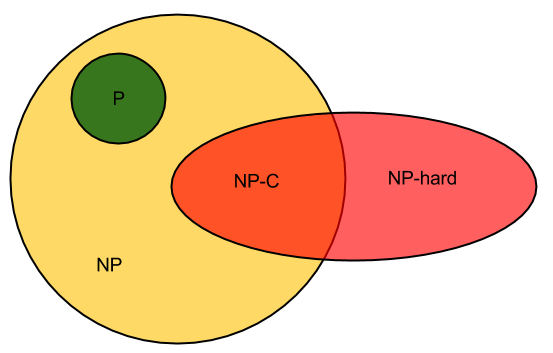
\includegraphics[height=7.5cm]{./chapters/litreview/complexity.png}
  \caption{The relationship between the various types of problem complexities.}
  \label{fig:complexity}
  \end{center}
\end{figure}
